% vim: spell spelllang=en:
%! TEX root = **/main.tex
%\documentclass[12pt, oneside]{article}
%\documentclass[draft, 12pt, oneside]{article}
\documentclass[final, 12pt, oneside]{article}
\usepackage[a4paper, left=2.5cm, right=2.5cm, top=2.5cm, bottom=2.5cm]{geometry}
%\usepackage[showframe, a4paper, left=2.5cm, right=2.5cm, top=2.5cm, bottom=2.5cm]{geometry}

\usepackage[T1]{fontenc}

%% Not needed with lualatex
%\usepackage[utf8]{inputenc} % Use unicode for input
%\usepackage{lmodern}

% With lualatex:
\usepackage{fontspec}
\setmonofont[Scale=MatchLowercase]{DejaVu Sans Mono}

\usepackage{microtype}

\usepackage{polyglossia}
\setdefaultlanguage{english}

\usepackage{hyphenat}

%% Bibliography:
\usepackage[
    backend=biber,
    style=numeric,
]{biblatex}
\DeclareNameAlias{default}{last-first}

%\DeclareQuoteAlias{spanish}{catalan}

\addbibresource{biblio.bib}
%% see:
%% https://www.sharelatex.com/learn/Bibliography_management_in_LaTeX#The_bibliography_file

% For cross references
\usepackage{color, xcolor}
\usepackage[breaklinks, colorlinks = true]{hyperref}
%hyperref configuration so that it doesn't contrast so much colorlinks,
\hypersetup{
   linkcolor={black},
   citecolor={black},
   urlcolor={blue!80!black}
}

\usepackage{mathtools}                    % amsmath + more
\usepackage{amsthm}                       % Theorem enviroment
\usepackage{amssymb}                      % More symbols
\usepackage{amstext}                      % Text inside mathenv

\usepackage{relsize}                      % Bigger math with mathlarger{___}
\usepackage{nicefrac}                     % nice fractions in one line

\usepackage[export]{adjustbox}            % Adjust table size
\usepackage{float}                        % Force tables and images position (H and H!)
\usepackage{wrapfig}                      % Wrap images like in HTML

%\usepackage{tabularx, colortbl, booktabs} % Better tables
%\usepackage{longtable}                    % Multiple page table
\usepackage{xltabular, colortbl, booktabs} % longtable + tabularx (has bug with booktabs: fix below)

% bug booktabs + xltabular
\makeatletter
\def\@BTrule[#1]{%
  \ifx\longtable\undefined
    \let\@BTswitch\@BTnormal
  \else\ifx\hline\LT@hline
    \nobreak
    \let\@BTswitch\@BLTrule
  \else
     \let\@BTswitch\@BTnormal
  \fi\fi
  \global\@thisrulewidth=#1\relax
  \ifnum\@thisruleclass=\tw@\vskip\@aboverulesep\else
  \ifnum\@lastruleclass=\z@\vskip\@aboverulesep\else
  \ifnum\@lastruleclass=\@ne\vskip\doublerulesep\fi\fi\fi
  \@BTswitch}
\makeatother

% Split cell in lines and more formating options inside table
\usepackage{array, multirow, multicol, makecell}

%\usepackage{subcaption}                     % Subfigures
%\usepackage[framemethod=tikz]{mdframed}     % Custom frames

\usepackage[bottom]{footmisc} % Footnotes at bottom of page

%\usepackage[alsoload=hep]{siunitx}          % SI units and uncertainties
%\sisetup{locale = FR}                       % Commas and so on for spanish
%\sisetup{separate-uncertainty=true}
%\sisetup{
  %per-mode=fraction,
  %fraction-function=\nicefrac
%}

%\usepackage{tikz}
%%\usetikzlibrary{arrows}
%%\usetikzlibrary{scopes}
%\usetikzlibrary{babel}

%% Custom Math operators (functions not in italic in math mode):
%\DeclareMathOperator{\cis}{cis}

% Set pages to landscape
% \usepackage{pdflscape}
% \usepackage{afterpage}

% \usepackage{pdfpages}

\usepackage{comment}        % multiline comments

% \usepackage{pifont}         % some fancy symbols

\usepackage{xspace}         % to create commands with space at end

%\usepackage{listings}       % For code listings (prefer minted)
%\usepackage{minted}         % -shell-escape
%\definecolor{codeBg}{HTML}{FFFDE7}
%\setminted[r]{
%    %style=pastie,
%    frame=lines,
%    framesep=3mm,
%    linenos,
%    breaklines=true,
%    encoding=utf8,
%    fontsize=\footnotesize,
%    bgcolor=codeBg
%}

% \usepackage{pgfgantt}           % Gantt chart

\newcommand{\whitepage}{        % white page without adding to pagenumber
    \clearpage\thispagestyle{empty}\addtocounter{page}{-1} \newpage \clearpage
}
\newcommand{\ts}{\textsuperscript}

\usepackage{tocbibind}

\usepackage[justification=centering]{caption}

\usepackage[english]{cleveref}
\usepackage{csquotes}       % For bibliography quotations

\usepackage{subcaption}

\usepackage{dsfont}

\addbibresource{biblio_aleix.bib}
\addbibresource{biblio_victor.bib}
\addbibresource{biblio_albert.bib}

\title{
    GCS - Quantum Encryption Report
}
\author{
Aleix Boné Ribó\\
Javier Cabrera Rodríguez\\
Victor Guardia Horcajada\\
Albert Mercadé Plasencia
}
\date{
    \today
}

\begin{document}

% vim: spell spelllang=en:
%! TEX root = **/main.tex

% Cover with title of work, name of course, data and list of working
% team members by alphabetical order of family name

\thispagestyle{empty}
\clearpage
\setcounter{page}{-1}

\begin{titlepage}
{
    \centering
    \null
    \vfill
    {\Large GCS\par}
    \vspace{2em}
    {\Huge \bfseries
        Quantum Computing Report
    \par}
    \vspace{2em}
    {\large \scshape
        \today
    \par}
    \vfill
\begin{center}

\end{center}
    \vspace{3cm}

    \vfill
    {\raggedleft \large
Aleix Boné Ribó\\
Javier Cabrera Rodríguez\\
Victor Guardia Horcajada\\
Albert Mercadé Plasencia
        \par}
}
\end{titlepage}


\tableofcontents

\setlength{\parskip}{1em}

\pagebreak
\section{Introduction}%
\label{sec:introduction}

In this report we attempt to give an overview of the current state of quantum
cryptography. First, we’ll look at the three most common pre-quantum algorithms:
Rivest–Shamir–Adleman (RSA), Elliptic curve cryptography (ECC) and Advanced
Encryption Standard (AES). We’ll examine their history, how they work and how
they will be affected by the advent of quantum computing.

In second place, we’ll present the most % TODO

Lastly, we’ll investigate what is the current state of quantum cryptography, how
it is being applied at present and what the future in this field looks like.


\pagebreak
\section{Can current common cryptographic methods survive the quantum world}

\subsection{Rivest–Shamir–Adleman (RSA)}

\subsubsection{History}

The concept of public-key cryptography was first introduced by Diffie and
Hellman in 1976 and is one of the most significant advances in cryptography.
They proved unnecessary that both parties in a communication meet beforehand to
agree on which methods to use for encoding and decoding the messages without
jeopardizing their privacy. Only one year later, in 1977, Rivest, Shamir and
Adlemen (RSA) published one of the first implementations of this idea through
their RSA algorithm \cite{rivest_method_1978}. Since then, it has become one of the most popular
cryptographic algorithms, used most notably in TLS and SSH.

\subsubsection{How it works}

First we’ll start by understanding how public-key cryptography works, as RSA is
a particular case of it, and then we’ll show the peculiarities of RSA's
encryption and decryption methods.

In public key cryptography, each user has a public encryption procedure $E$ and a
secret decryption procedure $D$. These procedures have the following four
properties:

\begin{enumerate}
    \item Decrypting the encrypted message $M$, produces $M$ i.e. $D(E(M)) = M$.
    \item Both are easy to compute.
    \item Making $E$ publicly available doesn't reveal in any way how to compute $D$.
    \item If a message $M$ is decrypted and then encrypted, $M$ is the result i.e. $E(D(M)) = M$.
\end{enumerate}

Having these properties in mind, let's imagine a communication between two very
famous users in cryptography, Alice ($A$) and Bob ($B$). Each of them have their own
public and private keys to encrypt and decrypt messages, respectively.

If Alice wants to send Bob a private message, first she will have to retrieve
from Bob's public encryption procedure $E_B$ and encrypt the message $M$ producing
the ciphered text $C$, which no one, other than Bob, can decipher because of
property 2. Then she will send $C$ to Bob, who, using his private decryption
procedure $D_A$, will decipher $C$ to obtain $M$, making use of property 1. As we have
seen, Alice has been able to send the message to Bob without previously agreeing
on any encryption and decryption methods and all through an insecure channel, as
any eavesdropper who intercepts the message won't be able to decrypt it, in
practice.

Through property 4, RSA is able to provide signatures that are message and
signer dependent as well, which allow users to prove who sent what message. If
Bob wants to send Alice a signed message, Bob will first compute his signature
$S=D_B(M)$ using his private procedure. He then encrypts $S$ using $E_A$ to send the
signature securely. When Alice receives the message, she obtains $S$ by using
$D_A$,
and then, using $E_B$, she is able to decipher the original message. This way,
Alice can prove that Bob sent the message, as no other person could have created
$S=D_B(M)$ and she can't modify the message, as she can't create the complementary
signature without Bob's private key.

The distinctiveness of RSA resides in how $E$ and $D$ are calculated, which
leverages the fact that back in 1977, and still today, the factorization of
large semiprime numbers (product of two primes) is in practice impossible. Each
user has a public key $(e, n)$ and a private key $(d,n)$, which are used to encrypt
and decrypt the message respectively. To encrypt:

\begin{equation}
    C \equiv E(M) \equiv M^e \quad mod \, n
\end{equation}

The receiver uses his private key $(d,n)$ to decipher the code this way:

\begin{equation}
    M \equiv D(C) \equiv C^d \quad mod \, n
\end{equation}

$n$, $e$ and $d$ are calculated the following way:
\begin{enumerate}
    \item Choose two random, very large prime numbers $p$ and $q$, and calculate $n = p \cdot q$.
    \item Select a number $d$ to be a large, random integer that is relatively prime to $(p-1)(q-1)$.
    \item Finally, $e$ can be computed using $p$, $q$ and $d$ to be the multiplicative inverse of $d$ modulo $(p-1)(q-1)$.
\end{enumerate}

The correctness of the deciphering algorithm $D(C)$ can be proved by Fermat's Little Theorem.

\subsubsection{How Quantum Computing affects it}

As mentioned before, RSA exploits the fact that while factoring large,
semiprime integers is technically possible, with today’s computational
power it would take an extremely long time, as the algorithms are
sub-exponential. As a matter of fact, it would take around 300 trillion
years to break a 2048 bit RSA encryption key 
\cite{andreas_baumhof_breaking_2019}. However, Peter Shor found
in 1994 that using quantum computers semiprime numbers can be factored
in polynomial time. Using Shor’s algorithm with 4099 perfectly stable
qubits, 2048-RSA would be broken in just 10 seconds. 

Today we don’t have a quantum computer with that many qubits or with
that quality of qubits for that matter. The largest quantum computer to
date is Google’s Bristlecone with 72 qubits and a 0.6\% error rate. 
Furthermore, the largest number that has been factored by a quantum 
computer is 35, a 6 digit number, very far off 2048 bits.

Nonetheless, last year two researchers published a paper in which they 
explained how to factor a 2048 bit RSA key in 8 hours using 20 million 
noisy qubits \cite{gidney_how_2019}. While 20 million qubits are many 
more than what is 
available today, for the first time a system that doesn’t use perfect 
qubits has been devised. Although there isn’t an imminent threat to RSA 
encryption, it isn’t a perfect algorithm and the supposition that very 
large, semiprime numbers can’t be factored in practice will be false in 
the coming decades. Thus, in a post-quantum world RSA will be 
broken, however large the key becomes, and therefore will no longer be 
secure.



\pagebreak
\subsection{Elliptic Curve Cryptography (ECC)}

\subsubsection{History}

ECC is a form of public key cryptography (or asymmetric) based on the complexity
of computing discrete logarithms in elliptic curve groups. (Elliptic Curve
Discrete Logarithm Problem).

Although elliptic curves have been studied since the work of Diophantus in the
second century A.D., its use in cryptography was not discovered until 1984.
Victor Miller and Neal Koblitz proposed two different methods to apply elliptic
curves to cryptography. \cite{barsagade_overview_2014}

The main attractiveness of ECC is that unlike with RSA, there are no known
sub-exponential time algorithms to solve ECDLP for properly chosen elliptic
curves. This makes it possible to have similar security with smaller parameters.
Moreover the computations needed to encrypt and decrypt are faster.

For instance, if we consider a standard 256bit ECDSA, the computing power needed
to crack with known algorithms is equivalent to a 3072 bit RSA.
\cite{roetteler_quantum_2017}

Nowadays, ECC is used all around the internet from TLS, SSH, Bitcoin, national
ID cards, the Tor anonymity network, and WhatsApp among others. Along with RSA,
ECC has become one of the cornerstones of the internet as we know it today.

\subsubsection{How it works}

An elliptic curve is a curve of the form: $y^2 = x^3 + ax + b$. To use it for
cryptographic purposes we have to agree on certain parameters called Domain
parameters: $(p,b,a,G,n,h)$. $p$ is the size of the field, $a,b$ are the curve
parameters, $G$ is the generator and $n$ its order ($\min(n)$ st $ n \times G$
is normally prime), $h$ is computed from $n$ and $G$. These parameters are hard
to compute and they are normally obtained from standards (standard curves).

Given a curve with domain parameters $(p,b,a,G,n,h)$, we can implement an
elliptic version of Diffie Hellman public key algorithm as follows:

Our public key will be the point $Q = d * G$ obtained by multiplying $G$ by our
private key $d$ (random number in the interval $[1, n-1]$) over the filed
$\mathds{F}_p$.

Consider now the scenario of Alice and Bob each one with their public and
private keys ($Q_A, d_A, Q_B, d_B$). They point $(x_a, y_a) = d_A * Q_B$ is
equal to $(x_b, y_b) = d_B * Q_A$ since $d_a * Q_B = d_a * d_b * G$. Therefore
this point can be used as a secret shared key. Although we can use the value of
the secret key as it is, most implementations hash its result for further
security.

It is important to note that if one of the parties gives a public key $Q$ that
is not part of the curve field, it can leak information about the private key of
the other and with sufficient malicious keys even obtain their private key. So
there must be a check that the points given are part of the valid subgroup.
\cite{pernul_practical_2015}


\subsubsection{How quantum computing affects it}

Despite the fact that with the know traditional algorithms, ECC is far superior
to RSA in terms of security, against the threat of quantum computing it is
equally vulnerable.

Shor published 2 algorithms in his famous paper: "Polynomial-Time Algorithms for
Prime Factorization and Discrete Logarithms on a Quantum Computer".
\cite{shor_polynomial-time_1997} Which can be
used to crack RSA and ECC in polynomial time. However, the cost of those
algorithms differ vastly.

As shown by Roetteler et al. (2017), ECC 256 requires $10^{11}$  toffoli gates
whereas RSA 3072 requires $10^{13}$. RSA provides greater security than ECC
using Shor's algorithms. However, there are improvements and optimizations that
can be applied to Shor's original prime factorization algorithm which reduce the
order of RSA by 100, making it comparable to ECC.

With current technology we are still very far away from being able to build a
quantum computer with sufficient qubits to crack either RSA or ECC, but progress
is being made rapidly, not only hardware wise but also on algorithms and
techniques (we went from needing 1 billion qubits to 20 million in the space of 7 years).
\cite{baumhof_are_2019}

\pagebreak

\subsection{Advanced Encryption Standard (AES)}

\subsubsection{History}

The Advanced Encryption Standard, originally submitted under the name
“Rijndael”, was submitted by Vincent Rijmen and Joan Daemen when in  1997 the
United States National Institute of Standards and Technology (NIST) called a
process to choose a successor for the aging and insecure DES algorithm, as an
alternative to the proposed 3DES variant, which was more secure but also quite
inefficient, and has nowadays been deprecated in favour of AES.

Among the fifteen competitors, aside from Rijndael, other noteworthy algorithms
were Serpent, Twofish and RC6, but taking into consideration several parameters,
like their cryptographic security, the complexity of their implementation and
their performance on different environments, Rijndael was chosen as the new
Advanced Encryption Standard.

\subsubsection{How it works}

AES is designed around an SP network, an algorithm based on substitutions and
permutations of the original data, repeated many times in so-called “rounds” to
increase security. The key is factored into the algorithm to ensure that it
can't be reversed without the key. While a detailed version of the AES algorithm
is out of the scope of this project, the following summarized version tries to
let the reader see the differences with the other algorithms exposed, and will
be used in the next section to discuss which attacks are possible and which are
not with quantum computers.

The algorithm assumes a 128 bit block size, which means that it expects a 128
bit input and returns a 128 bit output. Furthermore, it does not work over an
array, like other algorithms, but over a matrix of $4 \times 4$.

First, the original key, which can have a length of 128, 192 or 256 bits, is
expanded (or “scheduled”) into one “round key” for each round, plus an
additional initial key, which is xored with the input before the first round.

In each round, we substitute each byte of the input with another byte, according
to a lookup table defined in the standard.

\begin{figure}[H]
    \centering
    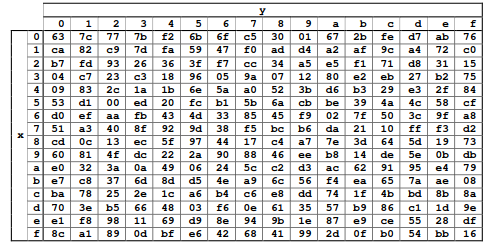
\includegraphics[width=0.7\textwidth]{images/aes-table}
\end{figure}

With the bytes substituted, the permutation part begins, rotating the contents
of each row by a different amount of columns, and multiplying each column by a
predefined matrix, with the intent of shuffling all the bits of the input.
Finally, the output is xored with the calculated round key. This process is
repeated during 10, 12 or 14 rounds (for 128, 196 and 256 bit-keys,
respectively), except for the column multiplication, skipped during the last
round.

\subsubsection{How Quantum Computing affects it}

As we have observed, no prime numbers are used on the algorithm. Therefore,
Shor's algorithm can not be applied to break AES. That does not mean that AES is
completely safe from quantum computers, however, as Grover's algorithm will
weaken (but not completely break) the security.

Grover's algorithm works by reversing a function that can be evaluated by a
quantum computer, whose input has $n$ possible values. While such a process would
ordinarily take $\mathcal{O}(n)$ evaluations of the function (what we would call
“brute-forcing”), using a quantum computer running Grover's algorithm we have a
high probability of finding the input which results in the chosen output with
only $\mathcal{O}(\sqrt{n})$ evaluations.

In the case of AES, for a key of length $k$ bits, brute-forcing it would take
$\mathcal{O}(2^k)$ steps. Therefore, 128 bits is currently considered very
secure, and 256 bits is regarded as nigh-unbreakable.

Grover's algorithm would reduce it to $\mathcal{O}\left(\sqrt{2^k}\right) =
\mathcal{O}\left({2^{k/2}}\right) $, effectively halving the security of the
key. Therefore, a 128-bit key would provide a security equivalent to what 64-bit
keys have without Quantum algorithms, which is thought to be insecure, but a
256-bit key would be equivalent to a 128-bit key, which is still considered
secure. Therefore, if it proved to be insufficiently secure, simply doubling the
key size effectively thwarts this kind of quantum attack.


\pagebreak
\section{Most important cryptographic methods in a post-quantum world}

\subsection{Error-correcting codes}
\subsubsection{Necessity of error correcting codes in a post-quantum world}

Error-correcting codes are a series of methods which aren't truly focused on
cybersecurity but rather the stability or the ability of it for not having
errors.

There is the possibility that interferences may occur during data messaging and
lead to incomplete or wrong data. In actual computers this type of code ensures
that a message can be sent in specific communications with a certain capability
to ensure that the message has been sent correctly or even ensure that if the
message is not sent correctly, we are able to correct the wrong part without the
message to be sent again. This is due to the addition of redundant information
in the message that helps verify its correct state.

As explained before, actual error-correcting codes cannot be applied to quantum
worlds, since the concept of the qubit is more unstable than the persistent bits
that they were meant for.

In the quantum world, error-correcting codes are extremely necessary since the
whole system tends to be very error prone. In fact, quantum computers weren't
considered viable without any way to prove that error-correcting codes could be
viable too. In 1995, Peter Shor proved that quantum error-correcting codes could
exist and a year later, researchers Dorit Aharonov and Michael Ben-Or proved
that these possible quantum error-correcting codes could theoretically push
error rates to almost zero.

\subsubsection{Error-correcting codes in practice}

In practice, quantum error correcting codes are still being researched and
developed, and there are multiple ways of ensuring the validity of data. The
actual objective of these methods is to ensure a single read qubit is truly
correct, since its volatility leads to a difficulty in knowing the true value of
a single qubit.

\pagebreak
\subsection{Hash-based cryptography}
\subsubsection{Necessity of hash-based cryptography in a post-quantum world}

While the evident usage of cryptographic algorithms is the encryption of data, an important part of the
digital world also relies on signatures, most of which are backed by cryptographic signing relying on
algorithms such as RSA, which, as it has been previously have analyzed, can be easily broken in a scenario 
where powerful-enough quantum are available.

Thus, it is needed to ensure that the signatures made can still be trusted even if classical asymmetric
algorithm are rendered obsolete, needing new algorithms to ensure this, and hash-based cryptography is a
good start point, as most of the algorithms in this field are quantum-proof, since Shor's algorithm can not
be applied to them. Grover's algorithm can still help find hash collisions, but, like in AES, can be easily
compensated doubling the hash size.

\subsubsection{Creating a signature from a hashing algorithm}

To create a signature, there are well-known algorithms that allow to sign a piece of information using any
proven hashing algorithm, like Lamport signatures and Winternitz signatures, but have a condition that
impedes their use: both are designed for One-Time Signature, and trying to reuse the signature will
void their security.

However, almost all practical usages of a signature key require that the signature can be reused. This
could be achieved by techniques like Merkle trees (or hash trees) which permit verifying that an element
is contained in a previously defined set.

Now, a brief explanation about Lamport signatures and Merkle trees is included to exemplify a possible
implementation of hash-based signatures. In those, $H$ will be the chosen hash function, as these
algorithms should be compatible with any function satisfying the hash properties.

\paragraph{Lamport signatures}
To sign a message $m$ of a length of 1 bit, a secret key with two components $(sk_0, sk_1)$ is generated.
This secret will have as a corresponding public key $(pk_0, pk_1)$, where $pk_x = H(sk_x)$.
Both are to be known by the recipient previous to the verification of the message. If $m = 0$, we release,
as a signature, $s = k_0$;  if $m = 1$, we release $s = k_1$ instead.

Thus, for a message $m$ with a
signature $s$, the signature can be easily verified by checking that $H(s) = pk_m$. One important
limitation of this algorithm is that to sign $N$ bits, $N$ keypairs have to be generated, and $N$
signatures have to be verified.

\paragraph{Merkle trees}
To improve the previous situation, we can generate a Merkle tree. To generate a Merkle tree of $N$
signing keys, we generate $N$ Lamport keypairs (other algorithms would work too), and build them into
a binary tree\footnote{Other trees may be used, but a binary one is the most common implementation}.
The non-leaf trees of the node will contain a hash of their children, recursively until the root node. Its
hash will be the public key. For every message we want to sign, we will provide the Lamport public key, the
signature, and the hashes of the nodes until the root.

To verify such a signature, the receiver would have to check the Lamport signature, and verify
that the public key was contained in the Merkle tree by checking each of the hashes provided as a
proof.

\pagebreak
\subsection{ Lattice cryptographic systems }

Lattice mathematical problems are ones of the most studied and prominent when
talking about cryptographic systems. These problems have been greatly studied
during the 19th century and there is a bast of studies related to this family of
problems.

Being a well known problem has led to an interest in using these problems as a
scheme for cryptographic systems.

\subsubsection{ What is a Lattice?  }

A Lattice is an infinite sequence of points in x dimensions that can be
calculated by a set of points called vectors. These set of vectors, called a
basis, if operated by a specific pattern, can form any point in the lattice.

As an example, we provide a 2 dimensional plane, in this plane we position an
origin point and define 2 new points defined by the vector from the origin. For
example, we could use $(2,0)$ and $(0,2)$.

\begin{figure}[H]
    \centering
    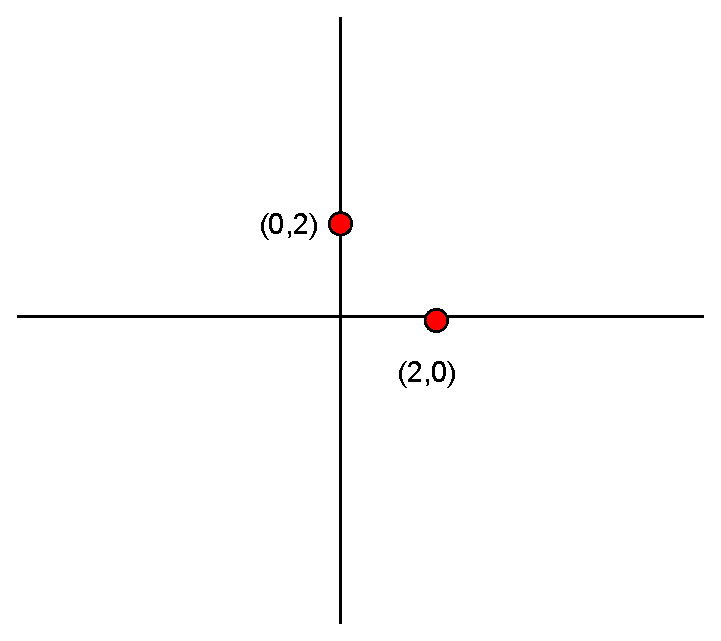
\includegraphics[width=0.4\textwidth]{images/lattice0}
\end{figure}

We can define a pattern in which to operate these vectors, that can be,
multiplying them by a natural number and summing up one or both of their
coordinates. This will lead to a new point.

In the next image we calculate a new point by multiplying the coordinates by 3
and adding them.

\begin{figure}[H]
    \centering
    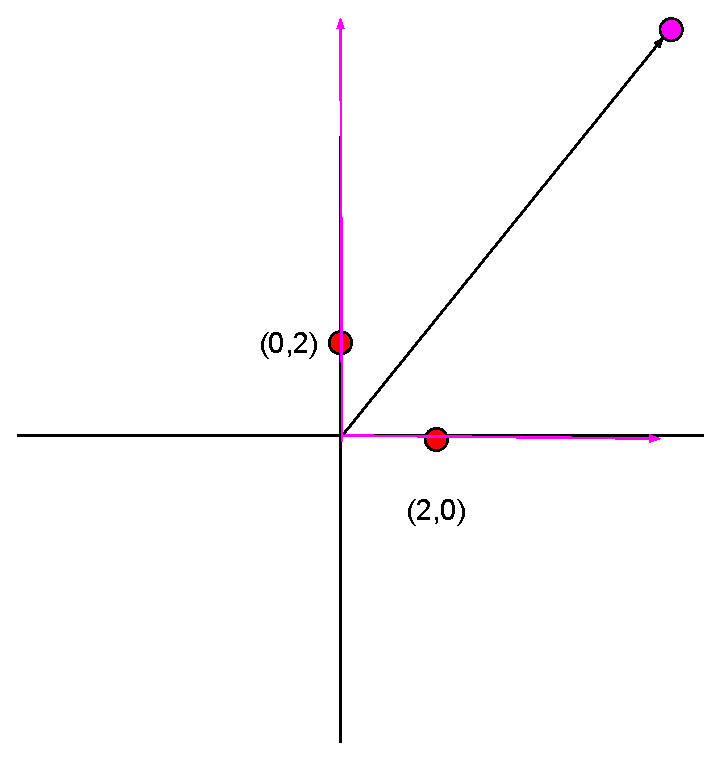
\includegraphics[width=0.4\textwidth]{images/lattice1}
\end{figure}

We can iterate more points with this pattern and we will get the Lattice.

\begin{figure}[H]
    \centering
    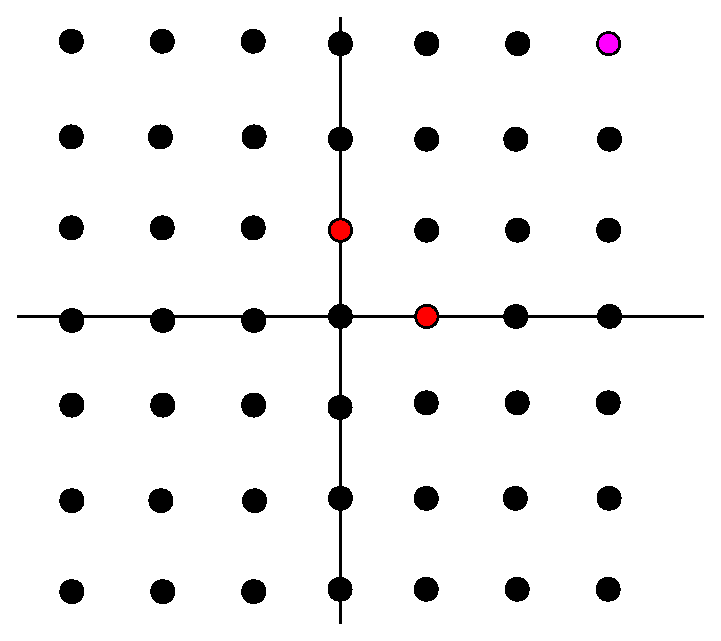
\includegraphics[width=0.4\textwidth]{images/lattice2}
\end{figure}

Example of another lattice:

\begin{figure}[H]
    \centering
    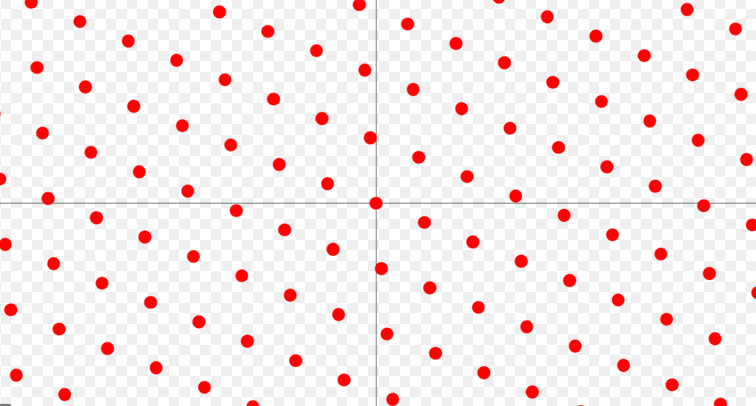
\includegraphics[width=0.5\textwidth]{images/lattice3}
\end{figure}

With this information, we now know that we can represent an $X$ dimension
lattice with a set of $X$ points, which is called a basis. A lattice can have
multiple bases, since for this example we could have perfectly used $(0,4)$ and
$(4,0)$ for example.

\subsubsection{What is interesting about Lattices?}

With lattices, we can elaborate a series of problems that can be easy to solve
if we use a small base like the one used in the example, but exponentially
difficult if we start using big numbers and an elevated quantity of dimensions,
like 10000.

One of the most famous and important problems is the Short Vector problem. Given
a long basis for some lattice $L$, find a point of the lattice which is as close
as possible to the origin point, but not equal. We can observe that with a small
basis, the problem might be easy, but with a big one, it becomes quite hard to
find a sufficiently small vector in multiple dimensions. This is the principal
argument which helps define lattice-based cryptographic systems as a good
candidate for the post-quantum era.

\subsubsection{Lattice-based cryptography advances}

In 1996, Miklós Atjai defined a cryptographic scheme that proved the
average-case hardness of lattice-based cryptographic schemes to be also
hard-case, which is known to be secure.

In the same year, NTRU was presented as a new public key cryptosystem based on
the lattice-based problems. This encryption system is still in development with
several advances in its performance and security.



\pagebreak
\subsection{Multivariate Public Key Cryptography (MVPKC)}

Multi variate public key cryptography is a method of public key cryptography
based on the NP-hardness of solving nonlinear equations over a finite field.
The fundamental principle of the method is rooted on algebraic geometry, a field
of mathematics that developed in the 20th century (and not numerical algebra or
elliptic curves). There are no known quantum algorithms that can break MVPKC
which makes it one of the candidates for post quantum cryptography methods.
\cite{ding_multivariate_2009}

The trapdoor way function of a MVPKC is a set of $m$ non linear polynomials with
$n$ variables:

$$ \mathcal{P} = (p_1(w_1, \dots, w_n), \dots, p_m(w_1, \dots, w_n))$$

The problem of finding values for $(w_1, \dots w_n)$ such that all polynomials
in $\mathcal{P}$ evaluate to 0 where all the variables and coefficients are in
the field $\mathds{F}_q$ is NP-hard.

There are various implementations of MVPKC, but the standard (bipolar) consists of using
the following public key: $\mathcal{P} = \mathcal{T} \circ \mathcal{Q} \circ \mathcal{S}$.
Where the sets of polynomials $\mathcal{T}, \mathcal{Q}, \mathcal{S}$ are the secret keys.

To encrypt we simple evaluate the polynomials:
\begin{equation}
    z = \mathcal{P}(w)
\end{equation}

To decrypt the data we have to know the inverse of $\mathcal{T}, \mathcal{Q}, \mathcal{S}$:
\begin{align*}
    y &= T^{−1}(z) \\
    x &= Q^{−1}(y) \\
    w &= S^{−1}(x)
\end{align*}

One of the main benefits of MVPKC over lattice and other post quantum
cryptography methods is that it takes less computing resources although the keys
are considerably larger (reaching Kbs in size). This makes it unsuitable for
small integrated devices with low memory.

\pagebreak
\section{Current state of quantum cryptography}

Quantum Key Distribution (QKD) has been proven to be an incorruptible system
for distributing encryption keys in perfect secrecy.  It's security is 
based on the foundations of quantum mechanics, as opposed to classical public
key distribution, which relies on the computational struggles of current
machines to solve the one-way trapdoor functions used. The first is 
theoretically proven to be unbreakable, while the second will become redundant
with the advent of capable quantum computers.
Because of this, there are many research groups, public and private,
working on implementations of QKD networks so that one day it can be used 
at a large scale. These include DARPA, SwissQuantum, EU's SECOQC, Los Alamos 
National Laboratory or China's QUESS.

In February of this year, a new record for QKD over optical fiber was established at 509 kilometers and with a secure key-rate seven times higher
than that of similar QKD systems \cite{qkd_509_km_2019}.

In parallel, there are already companies offering comercial QKD systems:
ID Quanitque (Switzerland), MagiQ Technologies (USA), QuintessenceLabs 
(Australia), SeQureNet (France) and Toshiba (Japan). However, this systems are 
complex and only used by large companies and government agencies.

Nonetheless, QKD is only half of the cryptography equation, as it only helps
with key distribution. We then have to consider the encryption techniques
in themselves, which can be cracked as well. It is known, and has been
theoretically proven that One-Time Pad (OTP) is unbreakable and therefore
a combination with QKD would result in a perfect encryption system. There
is in fact research being done on how to implement this type of system, for
example at the previously mentioned Los Alamos National Laboratory (USA).
In spite of all this promising expectations, OTP isn't very practical as it
requires true randomness to function. Furthermore, it requires that the size
of the key be at least as long as the message that it will encrypt.
For these reasons, it is very common
nowadays that QKD systems work with AES instead, as it provides all the security
in key distribution while AES, as we saw in a previous section, can be made
quantum resistant by simply doubling the key size.


\pagebreak
\section{Description of References}

\newcommand{\explainedcite}[2]{
\cite{#1} \fullcite{#1}

#2

\hrulefill
}

\hrulefill


\explainedcite{barsagade_overview_2014}{
    History of elliptic curves and its uses in cryptography
}

\explainedcite{baumhof_are_2019}{
    DEFCON talk on the current threat on cryptography and the progress on hardware
    and algorithmic research.
}

\explainedcite{ding_multivariate_2009}{
    Definition of MVPKC
}

\explainedcite{pernul_practical_2015}{
    Explanation of attack on badly implemented ECC cryptography that did not
    check the validity of the given points.
}

\explainedcite{roetteler_quantum_2017}{
    Cost of quantum algorithms to crack ECC.
}

\explainedcite{shor_polynomial-time_1997}{
    Peter Shor's algorithms for polynomial time cracking of RSA and ECC using
    quantum computers.
}

\explainedcite{singh_code_2000}{
    Book that talks about the history of cryptography. The last chapter focuses
    on quantum cryptography.
}

% VICTOR

\explainedcite{national_institute_of_standards_andtechnology_announcing_1997}{
    Publication of the AES requirements and call for algorithm.
}

\explainedcite{national_institute_of_standards_andtechnology_announcing_2001}{
    AES contest resolution.
}

\explainedcite{qutech_academy_grovers_2018}{
    Introduction to Grover's algorithm.
}

\explainedcite{wagner_is_2019}{
    Brief explanaition on AES quantum resiliency.
}

\explainedcite{green_2018}{
    Detailed explanation of Merkle Trees.
}

\explainedcite{minaud_2018}{
    Lamport signature explanaition and Merkle Tree overview.
}

% ALBERT

\explainedcite{gidney_how_2019}{
    How a quantum computer could break 2048-RSA in 8 hours.
}

\explainedcite{andreas_baumhof_breaking_2019}{
    How QC affects RSA
}

\explainedcite{rivest_method_1978}{
    Original RSA paper
}

\explainedcite{kelly_rsa_2009}{
    History of RSA
}

\explainedcite{qkd_509_km_2019} {
    
}




\pagebreak


\printbibliography




\end{document}
